\chapter{树}

\section{树}

\subsection{树(Tree)}

许多逻辑关系并不是简单的线性关系,在实际场景中,常常存在着一对多,甚至多对多的情况。树和图就是典型的非线性数据结构。\\

\begin{figure}[H]
	\centering
	\begin{tikzpicture}[
			level distance=2.5cm,
			level 1/.style={sibling distance=6cm},
			level 2/.style={sibling distance=2cm},
			level 3/.style={sibling distance=2cm}
		]
		\node {技术总监}
		child {
				node {项目经理A}
				child {node {员工A}}
				child {node {员工B}}
				child {node {员工C}}
			}
		child {
				node {项目经理B}
				child {node {员工D}}
				child {node {员工E}}
			};
	\end{tikzpicture}
	\caption{职级关系}
\end{figure}

这些结构都像自然界中的树一样,从同一个根衍生出许多枝干,再从每一个枝干衍生出许多更小的枝干,最后衍生出更多的叶子。\\

树是由$ n\ (n \ge 0) $个有限节点组成的一个具有层次关系的集合,当$ n = 0 $时称为空树。\\

在任意一个非空树中,有以下特点:

\begin{itemize}
	\item 有且有且仅有一个特定的结点称为根(root)。

	\item 当$ n > 1 $时,其余结点可分为$ m\ (m > 0) $个互不相交的有限集$ T_1, T_2, \dots, T_m $,其中每一个集合本身又是一棵树,并且称为根的子树(subtree)。
\end{itemize}

\vspace{0.5cm}

\subsection{树的术语}

\begin{figure}[H]
	\centering
	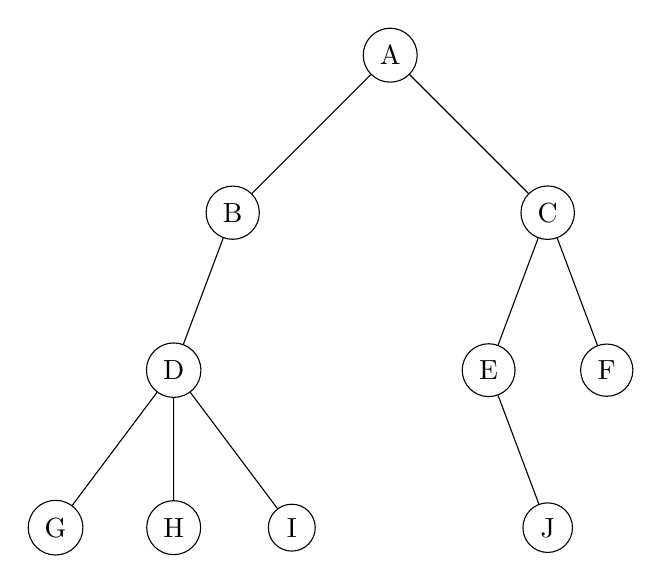
\begin{tikzpicture}[
			level distance=2cm,
			level 1/.style={sibling distance=4cm},
			level 2/.style={sibling distance=1.5cm},
			level 3/.style={sibling distance=1.5cm}
		]
		\node[circle,draw] {A}
		child {
				node[circle,draw] {B}
				child {
						node[circle,draw] {D}
						child {node[circle,draw] {G}}
						child {node[circle,draw] {H}}
						child {node[circle,draw] {I}}
					}
				child[missing] {}
			}
		child {
				node[circle,draw] {C}
				child {
						node[circle,draw] {E}
						child[missing] {}
						child {node[circle,draw] {J}}
					}
				child {node[circle,draw] {F}}
			};
	\end{tikzpicture}
	\caption{树}
\end{figure}

\begin{itemize}
	\item 根:没有父结点(parent)的结点。

	\item 内部结点(internal node):至少有一个子结点(child)的结点。

	\item 外部结点(external node) / 叶子结点(leaf node):没有子结点的结点。

	\item 度(degree):结点分支的个数。

	\item 路径(path):从根结点到树中某结点经过的分支构成了路径。

	\item 祖先结点(ancestors):包含父结点、父结点的父结点等。

	\item 子孙结点(descendants):包含子结点、子结点的子结点等。

	\item 深度(depth) / 高度(height):最大层级数。
\end{itemize}

\newpage

\section{二叉树}

\subsection{二叉树(Binary Tree)}

二叉树是树的一种特殊形式。二叉树的每个结点最多有两个孩子结点,即最多有2个,也可能只有1个,或者没有孩子结点。\\

二叉树结点的两个孩子结点,分别被称为左孩子(left child)和右孩子(right child)。这两个孩子结点的顺序是固定的,不能颠倒或混淆。\\

\begin{figure}[H]
	\centering
	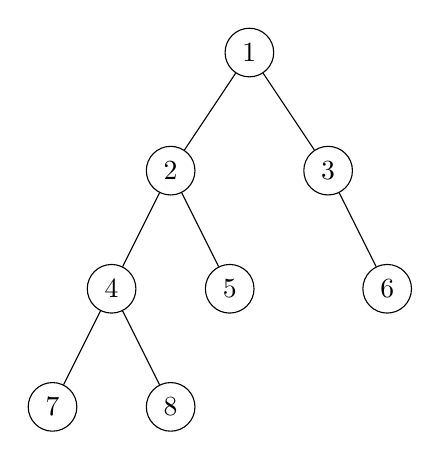
\begin{tikzpicture}[
			level distance=1.5cm,
			level 1/.style={sibling distance=2cm},
			level 2/.style={sibling distance=1.5cm},
			level 3/.style={sibling distance=1.5cm}
		]
		\node[circle,draw] {1}
		child {
				node[circle,draw] {2}
				child {
						node[circle,draw] {4}
						child {node[circle,draw] {7}}
						child {node[circle,draw] {8}}
					}
				child {node[circle,draw] {5}}
			}
		child {
				node[circle,draw] {3}
				child[missing] {}
				child {node[circle,draw] {6}}
			};
	\end{tikzpicture}
	\caption{二叉树}
\end{figure}

二叉树还有几种特殊的形式:

\subsubsection{左斜树(left skew tree) / 右斜树(right skew tree)}

只有左子树或只有右子树的二叉树。\\

\begin{figure}[H]
	\centering
	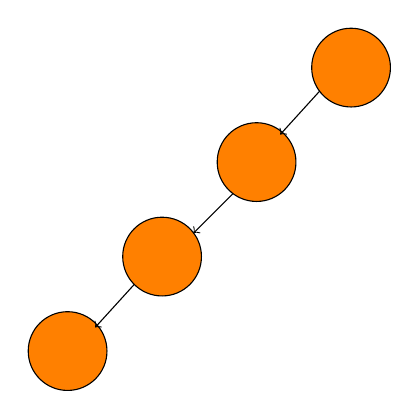
\begin{tikzpicture}
		\draw[fill=orange] (0,0) circle (0.5);
		\draw[fill=orange] (-1.2,-1.2) circle (0.5);
		\draw[fill=orange] (-2.4,-2.4) circle (0.5);
		\draw[fill=orange] (-3.6,-3.6) circle (0.5);

		\draw[->] (-0.4,-0.3) -- (-0.9,-0.85);
		\draw[->] (-1.5,-1.6) -- (-2,-2.1);
		\draw[->] (-2.75,-2.75) -- (-3.25,-3.3);
	\end{tikzpicture}
	\caption{左斜树}
\end{figure}

\subsubsection{满二叉树(full binary tree)}

所有非叶子结点都存在左右孩子,并且所有叶子结点都在同一层。\\

\begin{figure}[H]
	\centering
	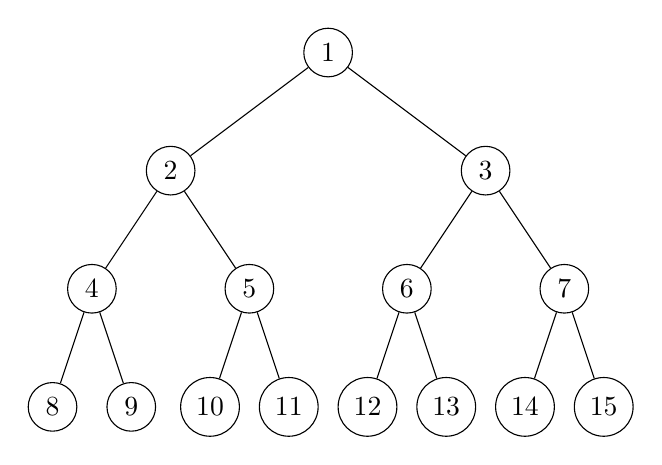
\begin{tikzpicture}[
			level distance=1.5cm,
			level 1/.style={sibling distance=4cm},
			level 2/.style={sibling distance=2cm},
			level 3/.style={sibling distance=1cm}
		]
		\node[circle,draw] {1}
		child {
				node[circle,draw] {2}
				child {
						node[circle,draw] {4}
						child {node[circle,draw] {8}}
						child {node[circle,draw] {9}}
					}
				child {
						node[circle,draw] {5}
						child {node[circle,draw] {10}}
						child {node[circle,draw] {11}}
					}
			}
		child {
				node[circle,draw] {3}
				child {
						node[circle,draw] {6}
						child {node[circle,draw] {12}}
						child {node[circle,draw] {13}}
					}
				child {
						node[circle,draw] {7}
						child {node[circle,draw] {14}}
						child {node[circle,draw] {15}}
					}
			};
	\end{tikzpicture}
	\caption{满二叉树}
\end{figure}

\subsubsection{完全二叉树}

对于一个有n个结点的二叉树,按层级顺序编号,则所有结点的编号从1到n,完全二叉树所有结点和同样深度的满二叉树的编号从1到n的结点位置相同。简单来说,就是除最后一层外,其它各层的结点数都达到最大,并且最后一层从右向左连续缺少若干个结点。\\

\begin{figure}[H]
	\centering
	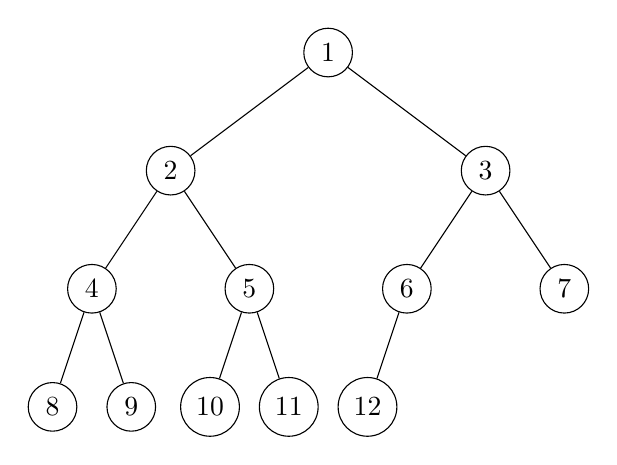
\begin{tikzpicture}[
			level distance=1.5cm,
			level 1/.style={sibling distance=4cm},
			level 2/.style={sibling distance=2cm},
			level 3/.style={sibling distance=1cm}
		]
		\node[circle,draw] {1}
		child {
				node[circle,draw] {2}
				child {
						node[circle,draw] {4}
						child {node[circle,draw] {8}}
						child {node[circle,draw] {9}}
					}
				child {
						node[circle,draw] {5}
						child {node[circle,draw] {10}}
						child {node[circle,draw] {11}}
					}
			}
		child {
				node[circle,draw] {3}
				child {
						node[circle,draw] {6}
						child {node[circle,draw] {12}}
						child[missing] {}
					}
				child {node[circle,draw] {7}}
			};
	\end{tikzpicture}
	\caption{完全二叉树}
\end{figure}

\vspace{0.5cm}

\subsection{二叉树的存储结构}

二叉树既可以通过链式存储,也可以使用数组存储:

\subsubsection{链式存储结构}

一个结点最多可以指向左右两个孩子结点,所以二叉树的每一个结点包含三个部分:

\begin{itemize}
	\item 存储数据的数据域data
	\item 指向左孩子的指针left
	\item 指向右孩子的指针right
\end{itemize}

\begin{figure}[H]
	\centering
	\begin{tikzpicture}
		\draw (0,0) rectangle (3,2);
		\draw (-1,-4) rectangle (-4,-2);
		\draw (4,-4) rectangle (7,-2);

		\draw (0,1) -- (3,1);
		\draw(1.5,1) -- (1.5,0);
		\draw (-4,-3) -- (-1,-3);
		\draw(-2.5,-4) -- (-2.5,-3);
		\draw (7,-3) -- (4,-3);
		\draw(5.5,-4) -- (5.5,-3);

		\draw (1.5,1.5) node{data};
		\draw (0.75,0.5) node{left};
		\draw (2.25,0.5) node{right};
		\draw (-2.5,-2.5) node{data};
		\draw (-3.25,-3.5) node{left};
		\draw (-1.75,-3.5) node{right};
		\draw (5.5,-2.5) node{data};
		\draw (4.75,-3.5) node{left};
		\draw (6.25,-3.5) node{right};

		\draw[->] (0.5,0.2) -- (-2,-2.5);
		\draw[->] (2.5,0.2) -- (5,-2.5);
	\end{tikzpicture}
	\caption{链式存储结构}
\end{figure}

\subsubsection{数组存储}

按照层级顺序把二叉树的结点放到数组中对应的位置上。如果某一结点的左孩子或右孩子空缺,则数组的相应位置也空出来。\\

\begin{figure}[H]
	\centering
	\begin{tikzpicture}[
			level distance=1.5cm,
			level 1/.style={sibling distance=4cm},
			level 2/.style={sibling distance=2cm},
			level 3/.style={sibling distance=1cm}
		]
		\node[circle,draw] {1}
		child {
				node[circle,draw] {2}
				child {
						node[circle,draw] {4}
						child[missing] {}
						child {node[circle,draw] {8}}
					}
				child {node[circle,draw] {5}}
			}
		child {
				node[circle,draw] {3}
				child[missing] {}
				child {node[circle,draw] {6}}
			};
	\end{tikzpicture}
\end{figure}

\begin{figure}[H]
	\centering
	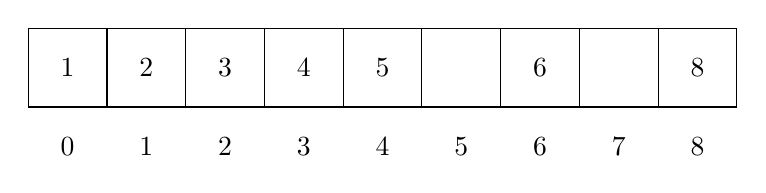
\begin{tikzpicture}[]
		\draw[-] (0,0) rectangle (9,1);
		\draw[-] (1,0) -- (1,1);
		\draw[-] (2,0) -- (2,1);
		\draw[-] (3,0) -- (3,1);
		\draw[-] (4,0) -- (4,1);
		\draw[-] (5,0) -- (5,1);
		\draw[-] (6,0) -- (6,1);
		\draw[-] (7,0) -- (7,1);
		\draw[-] (8,0) -- (8,1);

		\draw (0.5,0.5) node{1};
		\draw (1.5,0.5) node{2};
		\draw (2.5,0.5) node{3};
		\draw (3.5,0.5) node{4};
		\draw (4.5,0.5) node{5};
		\draw (6.5,0.5) node{6};
		\draw (8.5,0.5) node{8};

		\draw (0.5,-0.5) node{0};
		\draw (1.5,-0.5) node{1};
		\draw (2.5,-0.5) node{2};
		\draw (3.5,-0.5) node{3};
		\draw (4.5,-0.5) node{4};
		\draw (5.5,-0.5) node{5};
		\draw (6.5,-0.5) node{6};
		\draw (7.5,-0.5) node{7};
		\draw (8.5,-0.5) node{8};
	\end{tikzpicture}
	\caption{数组存储}
\end{figure}

采用数组存储可以更方便地定位二叉树的孩子结点和父结点。假设一个父结点的下标是parent,那么它的左孩子结点的下标就是2 * parent + 1,右孩子结点的下标就是2 * parent + 2。反过来,假设一个左孩子结点的下标是leftChild,那么它的父结点的下标就是(leftChild - 1) / 2。\\

但是,对于一个稀疏的二叉树来说,用数组表示法是非常浪费空间的。对于一种特殊的完全二叉树——二叉堆而言,就是使用数组进行存储的。

\newpage

\section{二叉树的遍历}

\subsection{二叉树的遍历}

在计算机程序中,遍历(traversal)本身是一个线性操作,所以遍历同样具有线性结构的数组或链表是一件轻而易举的事情。\\

反观二叉树,是典型的非线性数据结构,遍历时需要把非线性关联的结点转化成一个线性的序列,以不同的方式来遍历,遍历出的序列顺序也不同。\\

二叉树的遍历方式分为4种:

\begin{enumerate}
	\item 前序遍历(pre-order):访问根结点,遍历左子树,遍历右子树。

	\item 中序遍历(in-order):遍历左子树,访问根结点,遍历右子树。

	\item 后序遍历(post-order):遍历左子树,遍历右子树,访问根结点。

	\item 层次遍历(level-order):按照从根结点到叶子结点的层次关系,一层一层横向遍历。
\end{enumerate}

\vspace{0.5cm}

\subsection{前序遍历}

二叉树的前序遍历,首先访问根结点然后遍历左子树,最后遍历右子树。在遍历左、右子树时,仍然先访问根结点,然后遍历左子树,最后遍历右子树,如果结点为空则返回。\\

\begin{figure}[H]
	\centering
	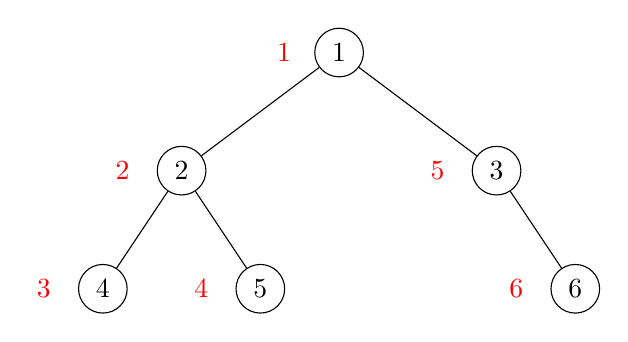
\begin{tikzpicture}[
			level distance=1.5cm,
			level 1/.style={sibling distance=4cm},
			level 2/.style={sibling distance=2cm},
			level 3/.style={sibling distance=1cm}
		]
		\node[circle,draw] {1}
		child {
				node[circle,draw] {2}
				child {
						node[circle,draw] {4}
					}
				child {
						node[circle,draw] {5}
					}
			}
		child {
				node[circle,draw] {3}
				child[missing] {}
				child {node[circle,draw] {6}}
			};

		\draw[color=red] (-0.7,0) node{1};
		\draw[color=red] (-2.75,-1.5) node{2};
		\draw[color=red] (-3.75,-3) node{3};
		\draw[color=red] (-1.75,-3) node{4};
		\draw[color=red] (1.25,-1.5) node{5};
		\draw[color=red] (2.25,-3) node{6};
	\end{tikzpicture}
	\caption{前序遍历}
\end{figure}

\mybox{前序遍历}

\begin{lstlisting}[language=C]
void preOrder(BST *root) {
    if(!root) {
        return;
    }
    printf("%d ", root->data);
    preOrder(root->left);
    preOrder(root->right);
}
\end{lstlisting}

\vspace{0.5cm}

\subsection{中序遍历}

二叉树的中序遍历,首先遍历左子树,然后访问根结点,最后遍历右子树,如果结点为空则返回。\\

\begin{figure}[H]
	\centering
	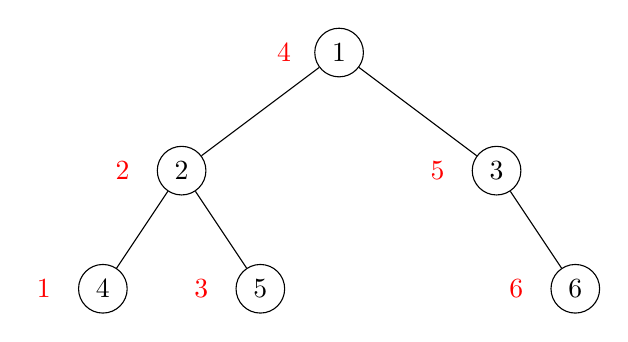
\begin{tikzpicture}[
			level distance=1.5cm,
			level 1/.style={sibling distance=4cm},
			level 2/.style={sibling distance=2cm},
			level 3/.style={sibling distance=1cm}
		]
		\node[circle,draw] {1}
		child {
				node[circle,draw] {2}
				child {
						node[circle,draw] {4}
					}
				child {
						node[circle,draw] {5}
					}
			}
		child {
				node[circle,draw] {3}
				child[missing] {}
				child {node[circle,draw] {6}}
			};

		\draw[color=red] (-0.7,0) node{4};
		\draw[color=red] (-2.75,-1.5) node{2};
		\draw[color=red] (-3.75,-3) node{1};
		\draw[color=red] (-1.75,-3) node{3};
		\draw[color=red] (1.25,-1.5) node{5};
		\draw[color=red] (2.25,-3) node{6};
	\end{tikzpicture}
	\caption{中序遍历}
\end{figure}

\mybox{中序遍历}

\begin{lstlisting}[language=C]
void inOrder(BST *root) {
    if(!root) {
        return;
    }
    inOrder(root->left);
    printf("%d ", root->data);
    inOrder(root->right);
}
\end{lstlisting}

\vspace{0.5cm}

\subsection{后序遍历}

二叉树的后序遍历,首先遍历左子树,然后遍历右子树,最后访问根结点,如果结点为空则返回。\\

\begin{figure}[H]
	\centering
	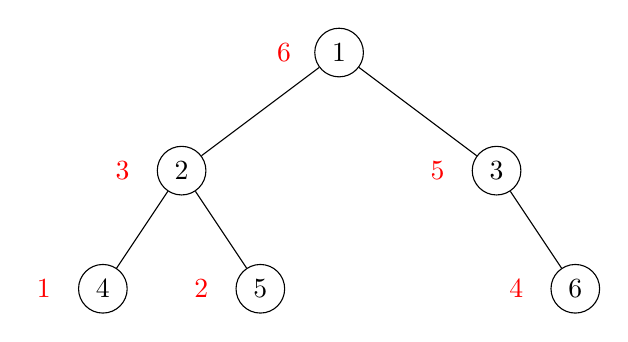
\begin{tikzpicture}[
			level distance=1.5cm,
			level 1/.style={sibling distance=4cm},
			level 2/.style={sibling distance=2cm},
			level 3/.style={sibling distance=1cm}
		]
		\node[circle,draw] {1}
		child {
				node[circle,draw] {2}
				child {
						node[circle,draw] {4}
					}
				child {
						node[circle,draw] {5}
					}
			}
		child {
				node[circle,draw] {3}
				child[missing] {}
				child {node[circle,draw] {6}}
			};

		\draw[color=red] (-0.7,0) node{6};
		\draw[color=red] (-2.75,-1.5) node{3};
		\draw[color=red] (-3.75,-3) node{1};
		\draw[color=red] (-1.75,-3) node{2};
		\draw[color=red] (1.25,-1.5) node{5};
		\draw[color=red] (2.25,-3) node{4};
	\end{tikzpicture}
	\caption{后序遍历}
\end{figure}

\mybox{后序遍历}

\begin{lstlisting}[language=C]
void postOrder(BST *root) {
    if(!root) {
        return;
    }
    postOrder(root->left);
    postOrder(root->right);
    printf("%d ", root->data);
}
\end{lstlisting}

\vspace{0.5cm}

\subsection{二叉树遍历非递归实现}

绝大多数可以用递归解决的问题,其实都可以用栈来解决,因为递归和栈都有回溯的特性。\\

以二叉树的中序遍历为例。当遇到一个结点时,就把它入栈,并去遍历它的左子树。当左子树遍历结束后,从栈顶弹出这个结点并访问它,然后按其右指针再去中序遍历该结点的右子树。\\

\mybox{中序遍历(非递归)}

\begin{lstlisting}[language=Java]
public void inOrderNonRecursive(BSTNode node) {
    Stack s = new Stack();
    while(node != null || !s.empty()) {
        // 一直向左并将沿途结点压入堆栈
        while(node != null) {
            s.push(node);
            node = node.left;
        }
        if(!s.empty()) {
            node = s.pop();					   //结点弹出堆栈
            System.out.println(node.data);		// 访问结点
            node = node.right;				   // 转向右子树
        }
    }
}
\end{lstlisting}

\vspace{0.5cm}

\subsection{层次遍历}

二叉树同一层次的结点之间是没有直接关联的,需要队列来辅助完成层序遍历。\\

层次遍历从根结点开始首先将根结点入队,然后开始循环执行以下操作直到队列为空:结点出队、访问该结点、其左右儿子入队。\\

\mybox{层次遍历}

\begin{lstlisting}[language=Java]
public void levelOrder(BSTNode node) {
    if(node == null) {
        return;
    }
    
    Queue q = new Queue();
    q.enqueue(node);
    while(!q.empty()) {
        node = q.dequeue();
        System.out.println(node.data);		// 访问结点
        if(node.left != null) {
            q.enqueue(node.left);
        }
        if(node.right != null) {
            q.enqueue(node.right);
        }
    }
}
\end{lstlisting}

\newpage

\section{二叉搜索树}

\subsection{二叉搜索树(Binary Search Tree)}

二叉搜索树,也称二叉查找树或二叉排序树,可以是一棵空树。\\

如果不为空树,那么二叉搜索树满足以下性质:

\begin{enumerate}
	\item 非空左子树的所有结点的值小于其根结点的值。
	\item 非空右子树的所有结点的值大于其根结点的值。
	\item 左、右子树均是二叉搜索树。
\end{enumerate}

\begin{figure}[H]
	\centering
	\begin{tikzpicture}[
			level distance=1.5cm,
			level 1/.style={sibling distance=4cm},
			level 2/.style={sibling distance=2cm},
			level 3/.style={sibling distance=1cm}
		]
		\node[circle,draw] {6}
		child {
				node[circle,draw] {3}
				child {
						node[circle,draw] {2}
						child {node[circle,draw] {1}}
						child[missing] {}
					}
				child {node[circle,draw] {4}}
			}
		child {
				node[circle,draw] {8}
				child {node[circle,draw] {7}}
				child {node[circle,draw] {9}}
			};
	\end{tikzpicture}
	\caption{二叉搜索树}
\end{figure}

\vspace{0.5cm}

\subsection{查找结点}

在二叉搜索树中查找一个元素从根结点开始,如果树为空,返回NULL。\\

如果树不为空,则将根结点的值和被查找的key值进行比较:

\begin{enumerate}
	\item 如果key值小于根结点的值,只需在左子树中继续查找。
	\item 如果key值大于根结点的值,只需在右子树中继续查找。
	\item 如果key值与根结点的值相等,查找成功。
\end{enumerate}

\mybox{查找结点(递归)}

\begin{lstlisting}[language=C]
Node* search(Node *root, dataType val) {
    if(!root) {
        return NULL;
    }
    if(val == root->data) {
        return root;
    } else if(val < root->data) {
        return search(root->left, val);
    } else {
        return search(root->right, val);
    }
}
\end{lstlisting}

由于非递归函数的执行效率高,可将尾递归(在函数最后才使用递归返回)的函数改为迭代函数。\\

\mybox{查找结点(迭代)}

\begin{lstlisting}[language=C]
Node* search(Node *root, dataType val) {
    if(!root) {
        return NULL;
    }  
    while(root) {
        if(root->data == val) {
            return root;
        } else if(val < root->data) {
            root = root->left;
        } else {
            root = root->right;
        }
    }
}
\end{lstlisting}

\vspace{0.5cm}

\subsection{查找最小值和最大值}

二叉搜索树中,最小值一定在树的最左分枝的叶子结点上,最大值一定在树的最右分枝的叶子结点上。\\

\mybox{查找最小值(递归)}

\begin{lstlisting}[language=C]
Node* findMin(Node *root) {
    if(!root) {
        return NULL;
    } else if(!root->left) {
        return root;
    } else {
        return findMin(root->left);		//沿左分枝继续查找
    }
}
\end{lstlisting}

\vspace{0.5cm}

\mybox{查找最大值(迭代)}

\begin{lstlisting}[language=C]
Node* findMax(Node *root) {
    if(!root) {
        return NULL;
    } 
    while(root->right) {
        root = root->right;
    }
    return root;
}
\end{lstlisting}

\vspace{0.5cm}

\subsection{插入结点}

在二叉搜索树中插入结点与查找的算法相似,需要找到插入的位置并将新结点插入。\\

\mybox{插入结点}

\begin{lstlisting}[language=C]
BST* insert(BST *root, dataType val) {
    // 空树,插入结点设为树根
    if(!root) {
        return init(val);
    }
    if(val < root->data) {
        root->left = insert(root->left, val);
    } else {
        root->right = insert(root->right, val);
    }
    return root;
}
\end{lstlisting}

\newpage

\section{哈夫曼树}

\subsection{哈夫曼树(Huffman Tree)}

树的每一个结点都可以拥有自己的权值(weight),假设二叉树有n个叶子结点,每个叶子结点都带有权值$ w_k $,从根结点到每个叶子结点的长度为$ l_k $,则树的带权路径长度(WPL, Weighted Path Length)为:

$$
	WPL = \sum_{k=1}^n w_k l_k
$$

哈夫曼树是由麻省理工学院的哈夫曼博士于1952年发明的,哈夫曼树是在叶子结点和权重确定的情况下,带权路径长度最小的二叉树,也被称为最优二叉树。\\

例如,有五个叶子结点,它们的权值为\{1, 2, 3, 4, 5\},用此权值序列可以构造出形状不同的多个二叉树。\\

\begin{figure}[H]
	\centering
	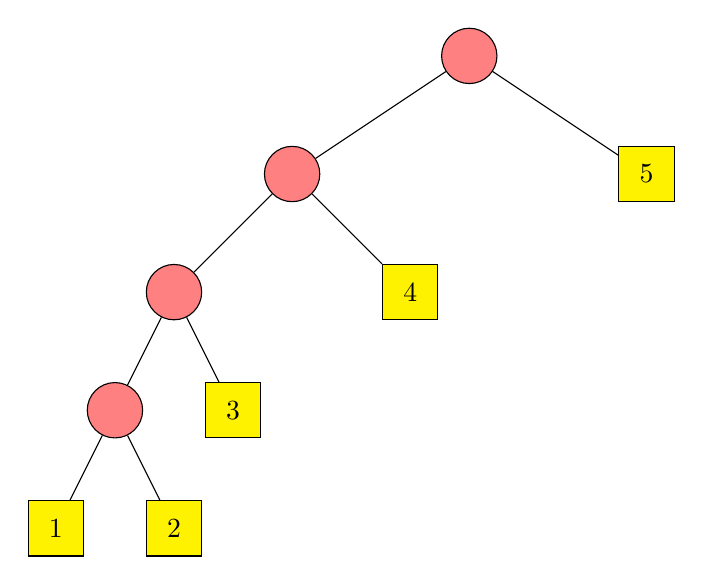
\begin{tikzpicture}[iv/.style={draw,fill=red!50,circle,minimum size=20pt,inner
					sep=0pt,text=black},ev/.style={draw,fill=yellow,rectangle,minimum
					size=20pt,inner sep=0pt,text=black}]
		\node[iv]{}
		child {node[iv]{}
				child {node[iv]{}
						child {node[iv]{}
								child {node[ev]{1}}
								child {node[ev]{2}}
							}
						child {node[ev]{3}}
					}
				child [missing]
				child {node[ev]{4}}
			}
		child [missing]
		child [missing]
		child {node[ev]{5}};
	\end{tikzpicture}
	\caption{WPL = 5 * 1 + 4 * 2 + 3 * 3 + 2 * 4 + 1 * 4 = 34}
\end{figure}

\begin{figure}[H]
	\centering
	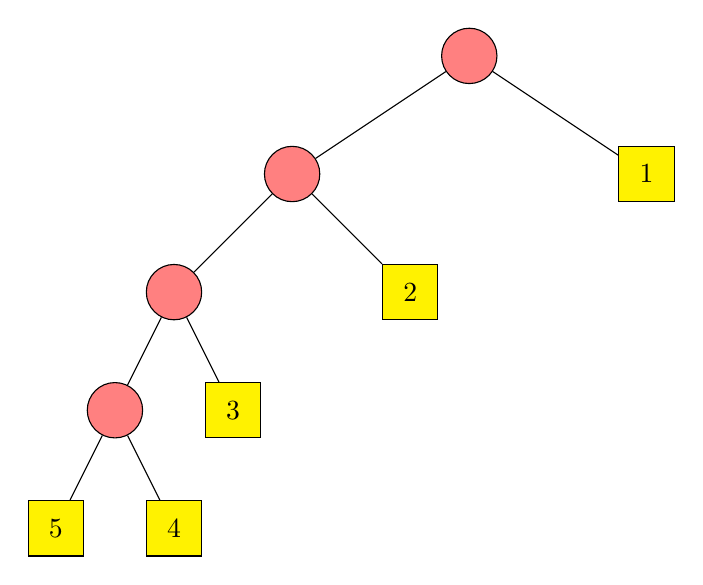
\begin{tikzpicture}[iv/.style={draw,fill=red!50,circle,minimum size=20pt,inner
					sep=0pt,text=black},ev/.style={draw,fill=yellow,rectangle,minimum
					size=20pt,inner sep=0pt,text=black}]
		\node[iv]{}
		child {node[iv]{}
				child {node[iv]{}
						child {node[iv]{}
								child {node[ev]{5}}
								child {node[ev]{4}}
							}
						child {node[ev]{3}}
					}
				child [missing]
				child {node[ev]{2}}
			}
		child [missing]
		child [missing]
		child {node[ev]{1}};
	\end{tikzpicture}
	\caption{WPL = 1 * 1 + 2 * 2 + 3 * 3 + 4 * 4 + 5 * 4 = 50}
\end{figure}

\begin{figure}[H]
	\centering
	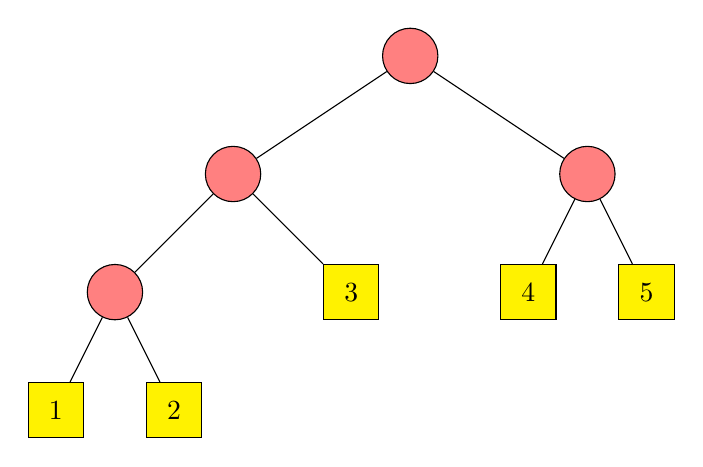
\begin{tikzpicture}[iv/.style={draw,fill=red!50,circle,minimum size=20pt,inner
					sep=0pt,text=black},ev/.style={draw,fill=yellow,rectangle,minimum
					size=20pt,inner sep=0pt,text=black}]
		\node[iv]{}
		child {node[iv]{}
				child {node[iv]{}
						child {node[ev]{1}}
						child {node[ev]{2}}
					}
				child [missing]
				child {node[ev]{3}}
			}
		child [missing]
		child [missing]
		child {node[iv]{}
				child {node[ev]{4}}
				child {node[ev]{5}}
			};
	\end{tikzpicture}
	\caption{WPL = 3 * 2 + 4 * 2 + 5 * 2 + 1 * 3 + 2 * 3 = 33}
\end{figure}

怎样才能保证构建出的二叉树带权路径长度最小呢?原则上,应该让权重小的叶子结点远离树根,权重大的叶子结点靠近树根。需要注意的是,同样叶子结点所构成的哈夫曼树可能不止一棵。\\

\subsection{哈夫曼树的构造}

哈夫曼树的构造方法就是每次把权值最小的两棵二叉树合并。\\

例如有6个叶子结点,权重依次是2、3、7、9、18、25。\\

第一步:把每一个叶子结点都当成一棵独立的树(只有根结点的树),这样就形成了一个森林。

\begin{figure}[H]
	\centering
	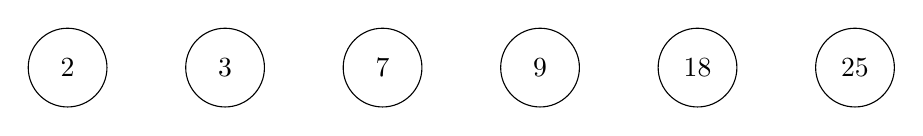
\begin{tikzpicture}
		\draw (0,0) circle (0.5) node{2};
		\draw (2,0) circle (0.5) node{3};
		\draw (4,0) circle (0.5) node{7};
		\draw (6,0) circle (0.5) node{9};
		\draw (8,0) circle (0.5) node{18};
		\draw (10,0) circle (0.5) node{25};
	\end{tikzpicture}
\end{figure}

第二步:从森林中移除权值最小的两个结点,生成父结点,父结点的权值是这两个结点权值之和,把父结点加入森林。重复该步骤,直到森林中只有一棵树为止。\\

\begin{figure}[H]
	\centering
	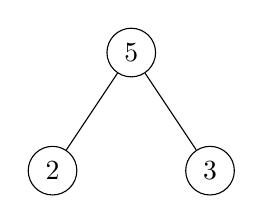
\begin{tikzpicture}[
			level distance=1.5cm,
			level 1/.style={sibling distance=2cm},
			level 2/.style={sibling distance=1.5cm},
			level 3/.style={sibling distance=1.5cm}
		]
		\node[circle,draw] {5}
		child {node[circle,draw] {2}}
		child {node[circle,draw] {3}};
	\end{tikzpicture}
	\caption{合并2和3}
\end{figure}

\begin{figure}[H]
	\centering
	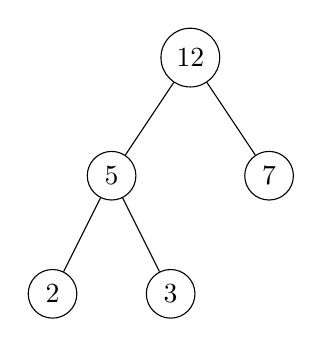
\begin{tikzpicture}[
			level distance=1.5cm,
			level 1/.style={sibling distance=2cm},
			level 2/.style={sibling distance=1.5cm},
			level 3/.style={sibling distance=1.5cm}
		]
		\node[circle,draw] {12}
		child {
				node[circle,draw] {5}
				child {node[circle,draw] {2}}
				child {node[circle,draw] {3}}
			}
		child {node[circle,draw] {7}};
	\end{tikzpicture}
	\caption{合并5和7}
\end{figure}

\begin{figure}[H]
	\centering
	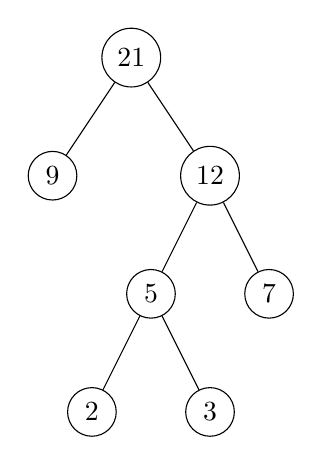
\begin{tikzpicture}[
			level distance=1.5cm,
			level 1/.style={sibling distance=2cm},
			level 2/.style={sibling distance=1.5cm},
			level 3/.style={sibling distance=1.5cm}
		]
		\node[circle,draw] {21}
		child {node[circle,draw] {9}}
		child {
				node[circle,draw] {12}
				child {
						node[circle,draw] {5}
						child {node[circle,draw] {2}}
						child {node[circle,draw] {3}}
					}
				child {node[circle,draw] {7}}
			};
	\end{tikzpicture}
	\caption{合并9和12}
\end{figure}

\begin{figure}[H]
	\centering
	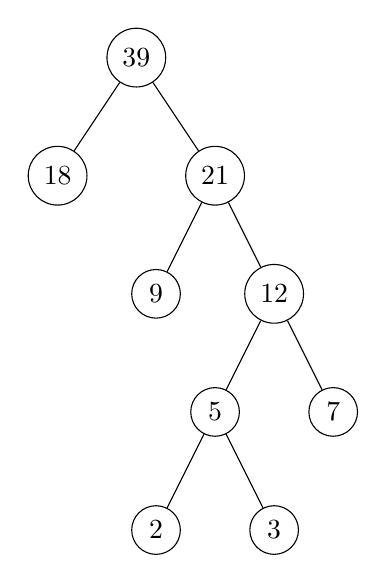
\begin{tikzpicture}[
			level distance=1.5cm,
			level 1/.style={sibling distance=2cm},
			level 2/.style={sibling distance=1.5cm},
			level 3/.style={sibling distance=1.5cm}
		]
		\node[circle,draw] {39}
		child {node[circle,draw] {18}}
		child {
				node[circle,draw] {21}
				child {node[circle,draw] {9}}
				child {
						node[circle,draw] {12}
						child {
								node[circle,draw] {5}
								child {node[circle,draw] {2}}
								child {node[circle,draw] {3}}
							}
						child {node[circle,draw] {7}}
					}
			};
	\end{tikzpicture}
	\caption{合并18和21}
\end{figure}

\begin{figure}[H]
	\centering
	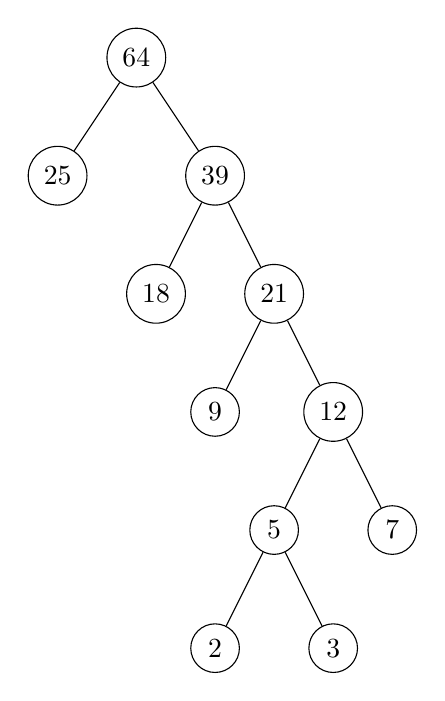
\begin{tikzpicture}[
			level distance=1.5cm,
			level 1/.style={sibling distance=2cm},
			level 2/.style={sibling distance=1.5cm},
			level 3/.style={sibling distance=1.5cm}
		]
		\node[circle,draw] {64}
		child {node[circle,draw] {25}}
		child {
				node[circle,draw] {39}
				child {node[circle,draw] {18}}
				child {
						node[circle,draw] {21}
						child {node[circle,draw] {9}}
						child {
								node[circle,draw] {12}
								child {
										node[circle,draw] {5}
										child {node[circle,draw] {2}}
										child {node[circle,draw] {3}}
									}
								child {node[circle,draw] {7}}
							}
					}
			};
	\end{tikzpicture}
	\caption{合并25和39}
\end{figure}

哈夫曼树有以下几个特点:

\begin{enumerate}
	\item 没有度为1的结点。
	\item 哈夫曼树的任意非叶结点的左右子树交换后仍是哈夫曼树。
	\item 对同一组权值,可能存在不同构的两棵哈夫曼树。
\end{enumerate}

\begin{figure}[H]
	\centering
	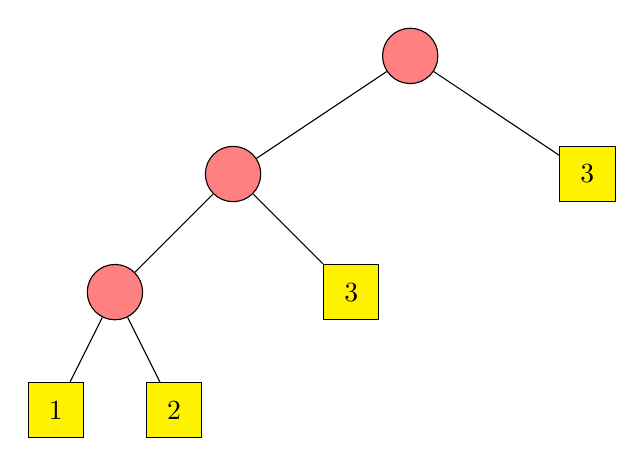
\begin{tikzpicture}[iv/.style={draw,fill=red!50,circle,minimum size=20pt,inner
					sep=0pt,text=black},ev/.style={draw,fill=yellow,rectangle,minimum
					size=20pt,inner sep=0pt,text=black}]
		\node[iv]{}
		child {node[iv]{}
				child {node[iv]{}
						child {node[ev]{1} }
						child {node[ev]{2}}
					}
				child [missing]
				child {node[ev]{3}}
			}
		child [missing]
		child [missing]
		child {node[ev]{3}};
	\end{tikzpicture}
	\caption{WPL = 3 * 1 + 3 * 2 + 1 * 3 + 2 * 3 = 18}
\end{figure}

\begin{figure}[H]
	\centering
	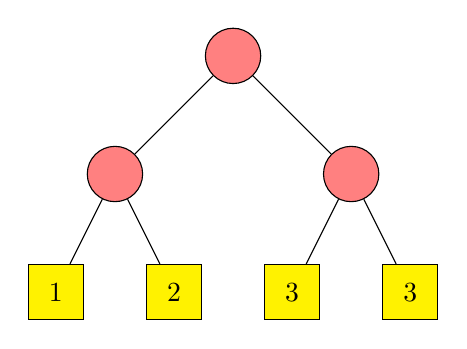
\begin{tikzpicture}[iv/.style={draw,fill=red!50,circle,minimum size=20pt,inner
					sep=0pt,text=black},ev/.style={draw,fill=yellow,rectangle,minimum
					size=20pt,inner sep=0pt,text=black}]
		\node[iv]{}
		child {node[iv]{}
				child {node[ev]{1}}
				child {node[ev]{2}}
			}
		child [missing]
		child {
				node[iv]{}
				child {node[ev]{3}}
				child {node[ev]{3}}
			};
	\end{tikzpicture}
	\caption{WPL = 1 * 2 + 2 * 2 + 3 * 2 + 3 * 2 = 18}
\end{figure}

\newpage

\section{哈夫曼编码}

\subsection{哈夫曼编码(Huffman Code)}

哈夫曼编码是一种高效的编码方式,在信息存储和传输过程中用于对信息进行压缩。要理解哈夫曼编码,需要从信息存储的底层逻辑讲起。\\

计算机不是人,它不认识中文和英文,更不认识图片和视频,它唯一认识的就是0(低电平)和1(高电平)。因此,计算机上一切文字、图象、音频、视频,底层都是用二进制来存储和传输的。\\

将信息转换成计算机能够识别的二进制形式的过程被称为编码。在ASCII码中,每一个字符表示成特定的8位二进制数。例如字符串APPLE表示成8位二进制编码为01000001 01010000 01010000 01001100 01000101。\\

显然,ASCII码是一种等长编码,也就是任何字符的编码长度都相等。等长编码的有点明显,因为每个字符对应的二进制编码长度相等,所以很容易设计,也很方便读写。但是计算机的存储空间以及网络传输的带宽是有限的,等长编码最大的缺点就是编码结果太长,会占用过多资源。\\

使用不等长编码,让出现频率高的字符用的编码短一些,出现频率低的字符编码长一些,可以使编码的总长度减小。但是不等长编码是不能随意设计的,如果一个字符的编码恰好是另一个字符编码的前缀,就会产生歧义的问题。\\

哈夫曼编码就是一种不等长的编码,并且任何一个字符的编码都不是另一个字符编码的前缀,因此可以无二义地进行解码,并且信息编码的总长度最小。\\

哈夫曼编码并非一套固定的编码,而是根据给定信息中各个字符出现的频次,动态生成最优的编码。哈夫曼编码的生成过程就用到了哈夫曼树。\\

例如一段信息里只有A、B、C、D、E、F这6个字符,出现的次数分别是2次、3次、7次、9次、18次、25次。通过把这6个字符当成6个叶子结点,将出现次数作为结点的权重,生成一颗哈夫曼树。将哈夫曼树中结点的左分支当做0、结点的右分支当做1,从哈夫曼树的根结点到每一个叶子结点的路径,都可以等价为一段二进制编码。\\

\begin{figure}[H]
	\centering
	\begin{forest}
		for tree={where n children={0}{ev}{iv},l+=8mm,
		if n=1{edge label={node [midway, left] {0} } }{edge label={node [midway, right] {1} } },}
		[
		[F]
			[
				[E]
					[
						[D]
							[
								[
										[A]
											[B]
									]
									[C]
							]
					]
			]
		]
	\end{forest}
\end{figure}

\begin{table}[H]
	\centering
	\setlength{\tabcolsep}{5mm}{
		\begin{tabular}{|c|c|}
			\hline
			\textbf{字符} & \textbf{编码} \\
			\hline
			\textbf{A}    & 11100         \\
			\hline
			\textbf{B}    & 11101         \\
			\hline
			\textbf{C}    & 1111          \\
			\hline
			\textbf{D}    & 110           \\
			\hline
			\textbf{E}    & 10            \\
			\hline
			\textbf{F}    & 0             \\
			\hline
		\end{tabular}
	}
	\caption{哈夫曼编码}
\end{table}

因为每一个字符对应的都是哈夫曼树的叶子结点,从根结点到这些叶子结点的路径并没有包含关系,最终得到的二进制编码自然也不会是彼此的前缀。

\newpage

\section{堆排序}

\subsection{堆(Heap)}

二叉堆本质上是一种完全二叉树,分为最大堆和最小堆两个类型。在最大堆中,任何一个父结点的值都大于等于它左右孩子结点的值。在最小堆中,任何一个父结点的值都小于等于它左右孩子结点的值。

\begin{figure}[H]
	\centering
	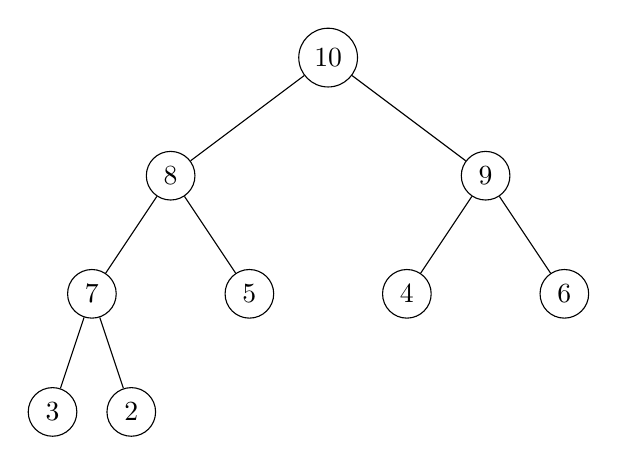
\begin{tikzpicture}[
			level distance=1.5cm,
			level 1/.style={sibling distance=4cm},
			level 2/.style={sibling distance=2cm},
			level 3/.style={sibling distance=1cm}
		]
		\node[circle,draw] {10}
		child {
				node[circle,draw] {8}
				child {
						node[circle,draw] {7}
						child {node[circle,draw] {3}}
						child {node[circle,draw] {2}}
					}
				child {node[circle,draw] {5}}
			}
		child {
				node[circle,draw] {9}
				child {node[circle,draw] {4}}
				child {node[circle,draw] {6}}
			};
	\end{tikzpicture}
	\caption{大顶堆}
\end{figure}

\begin{figure}[H]
	\centering
	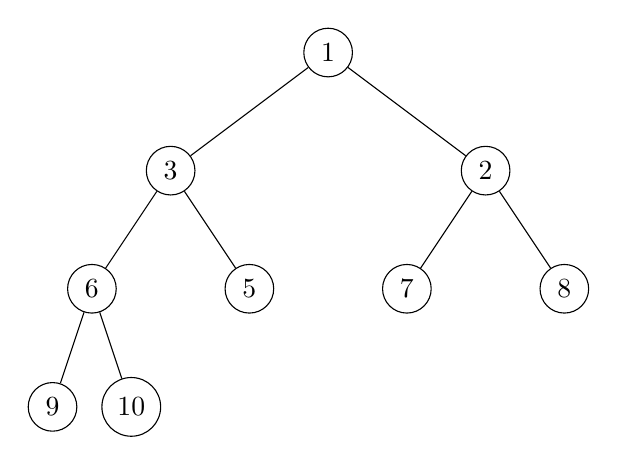
\begin{tikzpicture}[
			level distance=1.5cm,
			level 1/.style={sibling distance=4cm},
			level 2/.style={sibling distance=2cm},
			level 3/.style={sibling distance=1cm}
		]
		\node[circle,draw] {1}
		child {
				node[circle,draw] {3}
				child {
						node[circle,draw] {6}
						child {node[circle,draw] {9}}
						child {node[circle,draw] {10}}
					}
				child {node[circle,draw] {5}}
			}
		child {
				node[circle,draw] {2}
				child {node[circle,draw] {7}}
				child {node[circle,draw] {8}}
			};
	\end{tikzpicture}
	\caption{小顶堆}
\end{figure}

二叉堆的根结点称为堆顶,在最大堆中堆顶是整个堆中的最大元素,在最小堆中堆顶是整个堆中的最小元素。\\

在二叉堆中插入结点、删除结点、构造二叉堆的操作都基于堆的自我调整。\\

二叉堆虽然是一棵完全二叉树,但它的存储方式并不是链式存储,而是顺序存储。数组中,通过下标可以定位到结点的左右孩子,假设父结点的下标是parent,那么它的左孩子下标为2 * parent + 1、右孩子下标为2 * parent + 2。\\

\subsection{插入结点}

二叉堆的插入操作可以看成是结点上浮,当在堆中插入一个结点时,必须满足完全二叉树的标准,那么被插入结点的位置是完全二叉树的最后一个位置。在最大堆中,如果新结点的值大于它的父结点的值,则让新结点上浮,即和父结点交换位置。\\

堆的插入时间复杂度取决于树高为$ O(logn) $。\\

例如在大顶堆\{20, 15, 2, 14, 10\}中插入21:

\begin{figure}[H]
	\centering
	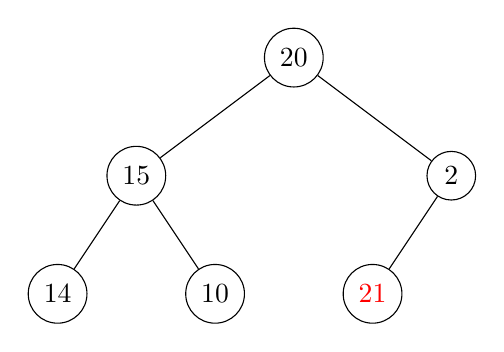
\begin{tikzpicture}[
			level distance=1.5cm,
			level 1/.style={sibling distance=4cm},
			level 2/.style={sibling distance=2cm},
			level 3/.style={sibling distance=1cm}
		]
		\node[circle,draw] {20}
		child {
				node[circle,draw] {15}
				child {node[circle,draw] {14}}
				child {node[circle,draw] {10}}
			}
		child {
				node[circle,draw] {2}
				child {node[circle,draw] {\textcolor{red}{21}}}
				child[missing] {}
			};
	\end{tikzpicture}
\end{figure}

\begin{figure}[H]
	\centering
	\begin{tikzpicture}[font=\ttfamily,
			array/.style={matrix of nodes,nodes={draw, minimum size=10mm, fill=green!30},column sep=-\pgflinewidth, row sep=0.5mm, nodes in empty cells,
					row 1/.style={nodes={draw=none, fill=none, minimum size=5mm}},
				}]

		\matrix[array] (array) {
			0  & 1  & 2 & 3  & 4  & 5                      \\
			20 & 15 & 2 & 14 & 10 & \textcolor{red}{21} \\
		};
	\end{tikzpicture}
\end{figure}

将新元素21与其父结点2比较,因为21 > 2,将21和2的位置交换:

\begin{figure}[H]
	\centering
	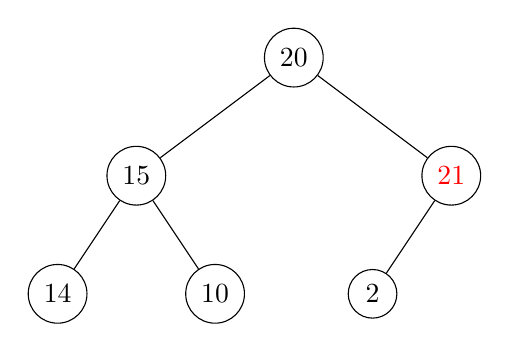
\begin{tikzpicture}[
			level distance=1.5cm,
			level 1/.style={sibling distance=4cm},
			level 2/.style={sibling distance=2cm},
			level 3/.style={sibling distance=1cm}
		]
		\node[circle,draw] {20}
		child {
				node[circle,draw] {15}
				child {node[circle,draw] {14}}
				child {node[circle,draw] {10}}
			}
		child {
				node[circle,draw] {\textcolor{red}{21}}
				child {node[circle,draw] {2}}
				child[missing] {}
			};
	\end{tikzpicture}
\end{figure}

\begin{figure}[H]
	\centering
	\begin{tikzpicture}[font=\ttfamily,
			array/.style={matrix of nodes,nodes={draw, minimum size=10mm, fill=green!30},column sep=-\pgflinewidth, row sep=0.5mm, nodes in empty cells,
					row 1/.style={nodes={draw=none, fill=none, minimum size=5mm}},
				}]

		\matrix[array] (array) {
			0  & 1  & 2                      & 3  & 4  & 5 \\
			20 & 15 & \textcolor{red}{21} & 14 & 10 & 2 \\
		};
	\end{tikzpicture}
\end{figure}

因为21 > 20,将21与20的位置交换:

\begin{figure}[H]
	\centering
	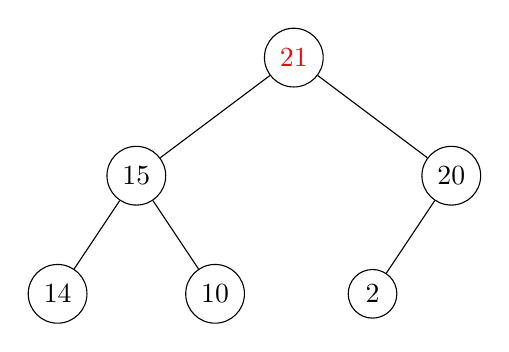
\begin{tikzpicture}[
			level distance=1.5cm,
			level 1/.style={sibling distance=4cm},
			level 2/.style={sibling distance=2cm},
			level 3/.style={sibling distance=1cm}
		]
		\node[circle,draw] {\textcolor{red}{21}}
		child {
				node[circle,draw] {15}
				child {node[circle,draw] {14}}
				child {node[circle,draw] {10}}
			}
		child {
				node[circle,draw] {20}
				child {node[circle,draw] {2}}
				child[missing] {}
			};
	\end{tikzpicture}
\end{figure}

\begin{figure}[H]
	\centering
	\begin{tikzpicture}[font=\ttfamily,
			array/.style={matrix of nodes,nodes={draw, minimum size=10mm, fill=green!30},column sep=-\pgflinewidth, row sep=0.5mm, nodes in empty cells,
					row 1/.style={nodes={draw=none, fill=none, minimum size=5mm}},
				}]

		\matrix[array] (array) {
			0                      & 1  & 2  & 3  & 4  & 5 \\
			\textcolor{red}{21} & 15 & 20 & 14 & 10 & 2 \\
		};
	\end{tikzpicture}
\end{figure}

\vspace{0.5cm}

\subsection{删除结点}

二叉堆的删除操作总是从堆的根结点删除元素。根结点被删除之后为了能够保证该树还是一棵完全二叉树,需要将完全二叉树的最后一个结点补到根结点的位置,让其继续符合完全二叉树的定义。二叉堆的删除结点操作可以看作是结点下沉。在最大堆中,如果新堆顶元素小于它的左右孩子中较大的那个结点,则与它的较大的子结点交换位置。\\

堆的删除时间复杂度取决于树高为$ O(logn) $。\\

例如删除大顶堆的堆顶元素20:

\begin{figure}[H]
	\centering
	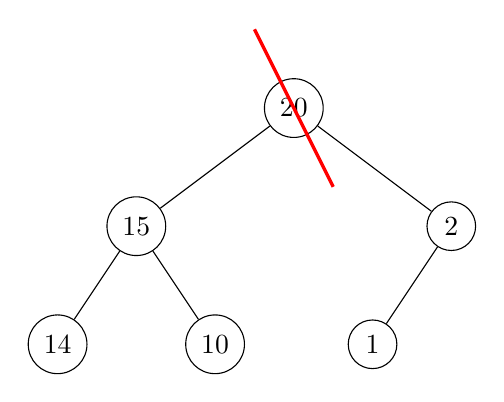
\begin{tikzpicture}[
			level distance=1.5cm,
			level 1/.style={sibling distance=4cm},
			level 2/.style={sibling distance=2cm},
			level 3/.style={sibling distance=1cm}
		]
		\node[circle,draw] {20}
		child {
				node[circle,draw] {15}
				child {node[circle,draw] {14}}
				child {node[circle,draw] {10}}
			}
		child {
				node[circle,draw] {2}
				child {node[circle,draw] {1}}
				child[missing] {}
			};

		\draw[very thick, red] (-0.5,1) -- (0.5,-1);
	\end{tikzpicture}
\end{figure}

\begin{figure}[H]
	\centering
	\begin{tikzpicture}[font=\ttfamily,
			array/.style={matrix of nodes,nodes={draw, minimum size=10mm, fill=green!30},column sep=-\pgflinewidth, row sep=0.5mm, nodes in empty cells,
					row 1/.style={nodes={draw=none, fill=none, minimum size=5mm}},
				}]

		\matrix[array] (array) {
			0                      & 1  & 2 & 3  & 4  & 5 \\
			\textcolor{red}{20} & 15 & 2 & 14 & 10 & 1 \\
		};
	\end{tikzpicture}
\end{figure}

移动最后一个结点到堆顶,使其满足二叉树的性质:

\begin{figure}[H]
	\centering
	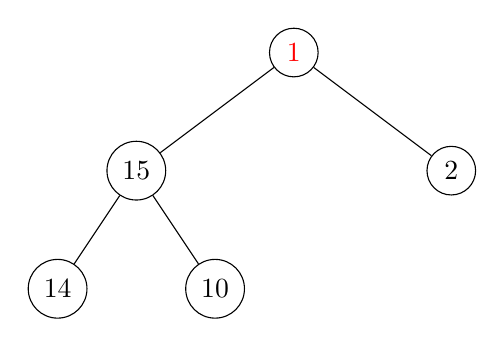
\begin{tikzpicture}[
			level distance=1.5cm,
			level 1/.style={sibling distance=4cm},
			level 2/.style={sibling distance=2cm},
			level 3/.style={sibling distance=1cm}
		]
		\node[circle,draw] {\textcolor{red}{1}}
		child {
				node[circle,draw] {15}
				child {node[circle,draw] {14}}
				child {node[circle,draw] {10}}
			}
		child {node[circle,draw] {2}};
	\end{tikzpicture}
\end{figure}

\begin{figure}[H]
	\centering
	\begin{tikzpicture}[font=\ttfamily,
			array/.style={matrix of nodes,nodes={draw, minimum size=10mm, fill=green!30},column sep=-\pgflinewidth, row sep=0.5mm, nodes in empty cells,
					row 1/.style={nodes={draw=none, fill=none, minimum size=5mm}},
				}]

		\matrix[array] (array) {
			0                      & 1  & 2 & 3  & 4  \\
			\textcolor{red}{1} & 15 & 2 & 14 & 10 \\
		};
	\end{tikzpicture}
\end{figure}

将堆顶元素1与其子结点比较,因为15 > 2,交换较大子结点15与1的位置:

\begin{figure}[H]
	\centering
	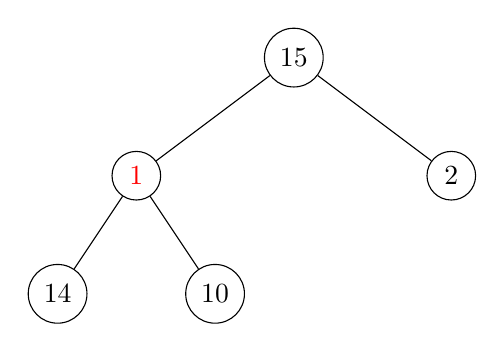
\begin{tikzpicture}[
			level distance=1.5cm,
			level 1/.style={sibling distance=4cm},
			level 2/.style={sibling distance=2cm},
			level 3/.style={sibling distance=1cm}
		]
		\node[circle,draw] {15}
		child {
				node[circle,draw] {\textcolor{red}{1}}
				child {node[circle,draw] {14}}
				child {node[circle,draw] {10}}
			}
		child {node[circle,draw] {2}};
	\end{tikzpicture}
\end{figure}

\begin{figure}[H]
	\centering
	\begin{tikzpicture}[font=\ttfamily,
			array/.style={matrix of nodes,nodes={draw, minimum size=10mm, fill=green!30},column sep=-\pgflinewidth, row sep=0.5mm, nodes in empty cells,
					row 1/.style={nodes={draw=none, fill=none, minimum size=5mm}},
				}]

		\matrix[array] (array) {
			0  & 1                      & 2 & 3  & 4  \\
			15 & \textcolor{red}{1} & 2 & 14 & 10 \\
		};
	\end{tikzpicture}
\end{figure}

继续将元素1与其子结点比较,因为14 > 10,交换较大子结点14与1的位置:

\begin{figure}[H]
	\centering
	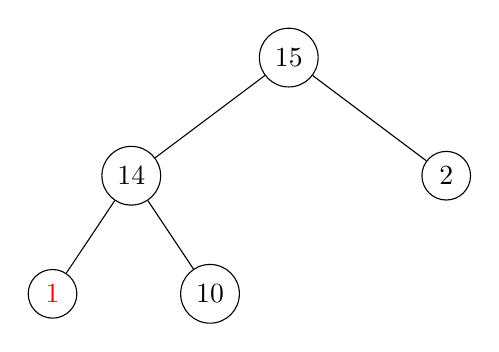
\begin{tikzpicture}[
			level distance=1.5cm,
			level 1/.style={sibling distance=4cm},
			level 2/.style={sibling distance=2cm},
			level 3/.style={sibling distance=1cm}
		]
		\node[circle,draw] {15}
		child {
				node[circle,draw] {14}
				child {node[circle,draw] {\textcolor{red}{1}}}
				child {node[circle,draw] {10}}
			}
		child {node[circle,draw] {2}};
	\end{tikzpicture}
\end{figure}

\begin{figure}[H]
	\centering
	\begin{tikzpicture}[font=\ttfamily,
			array/.style={matrix of nodes,nodes={draw, minimum size=10mm, fill=green!30},column sep=-\pgflinewidth, row sep=0.5mm, nodes in empty cells,
					row 1/.style={nodes={draw=none, fill=none, minimum size=5mm}},
				}]

		\matrix[array] (array) {
			0  & 1 & 2 & 3                      & 4  \\
			15 & 1 & 2 & \textcolor{red}{1} & 10 \\
		};
	\end{tikzpicture}
\end{figure}

\vspace{0.5cm}

\subsection{构建二叉堆}

构建二叉堆,就是把一个无序的完全二叉树调整为二叉堆,本质上就是让所有非叶子结点依次下沉。\\

例如将一个无序的完全二叉树构建成最小堆:

\begin{figure}[H]
	\centering
	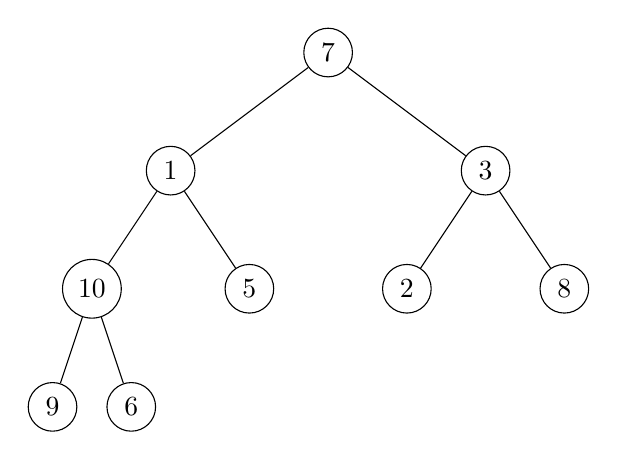
\begin{tikzpicture}[
			level distance=1.5cm,
			level 1/.style={sibling distance=4cm},
			level 2/.style={sibling distance=2cm},
			level 3/.style={sibling distance=1cm}
		]
		\node[circle,draw] {7}
		child {
				node[circle,draw] {1}
				child {
						node[circle,draw] {10}
						child {node[circle,draw] {9}}
						child {node[circle,draw] {6}}
					}
				child {node[circle,draw] {5}}
			}
		child {
				node[circle,draw] {3}
				child {node[circle,draw] {2}}
				child {node[circle,draw] {8}}
			};
	\end{tikzpicture}
\end{figure}

首先从最后一个非叶子结点开始,结点10下沉:

\begin{figure}[H]
	\centering
	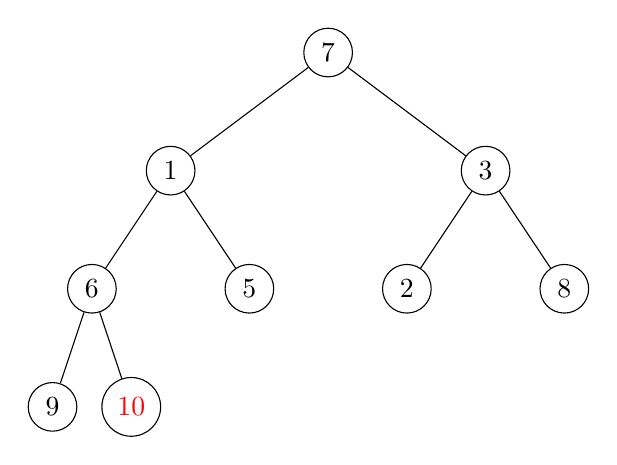
\begin{tikzpicture}[
			level distance=1.5cm,
			level 1/.style={sibling distance=4cm},
			level 2/.style={sibling distance=2cm},
			level 3/.style={sibling distance=1cm}
		]
		\node[circle,draw] {7}
		child {
				node[circle,draw] {1}
				child {
						node[circle,draw] {6}
						child {node[circle,draw] {9}}
						child {node[circle,draw] {\textcolor{red}{10}}}
					}
				child {node[circle,draw] {5}}
			}
		child {
				node[circle,draw] {3}
				child {node[circle,draw] {2}}
				child {node[circle,draw] {8}}
			};
	\end{tikzpicture}
\end{figure}

接着处理倒数第二个非叶子结点,结点3下沉:

\begin{figure}[H]
	\centering
	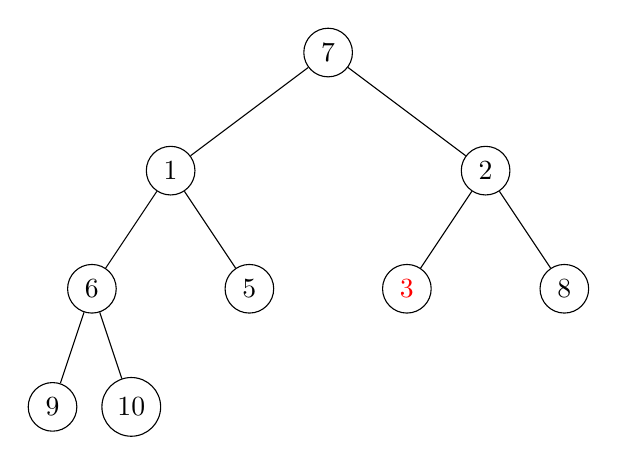
\begin{tikzpicture}[
			level distance=1.5cm,
			level 1/.style={sibling distance=4cm},
			level 2/.style={sibling distance=2cm},
			level 3/.style={sibling distance=1cm}
		]
		\node[circle,draw] {7}
		child {
				node[circle,draw] {1}
				child {
						node[circle,draw] {6}
						child {node[circle,draw] {9}}
						child {node[circle,draw] {10}}
					}
				child {node[circle,draw] {5}}
			}
		child {
				node[circle,draw] {2}
				child {node[circle,draw] {\textcolor{red}{3}}}
				child {node[circle,draw] {8}}
			};
	\end{tikzpicture}
\end{figure}

倒数第三个非叶子结点1无需移动。\\

最后处理倒数第四个非叶子结点7下沉:

\begin{figure}[H]
	\centering
	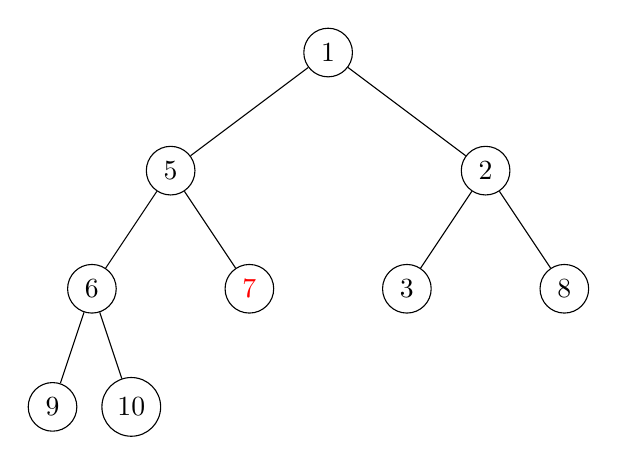
\begin{tikzpicture}[
			level distance=1.5cm,
			level 1/.style={sibling distance=4cm},
			level 2/.style={sibling distance=2cm},
			level 3/.style={sibling distance=1cm}
		]
		\node[circle,draw] {1}
		child {
				node[circle,draw] {5}
				child {
						node[circle,draw] {6}
						child {node[circle,draw] {9}}
						child {node[circle,draw] {10}}
					}
				child {node[circle,draw] {\textcolor{red}{7}}}
			}
		child {
				node[circle,draw] {2}
				child {node[circle,draw] {3}}
				child {node[circle,draw] {8}}
			};
	\end{tikzpicture}
\end{figure}

最终一棵无序完全二叉树就调整成了一个最小堆。\\

\subsection{堆排序(Heap Sort)}

有了二叉堆的构建、删除和自我调节,实现堆排序就是水到聚成了。当删除一个最大堆的堆顶后(并不是完全删除,而是替换到堆的最后面),经过自我调节,第二大的元素就会被交换上来,成为最大堆的新堆顶。\\

首先将待排序数组构建成大顶堆:

\begin{figure}[H]
	\centering
	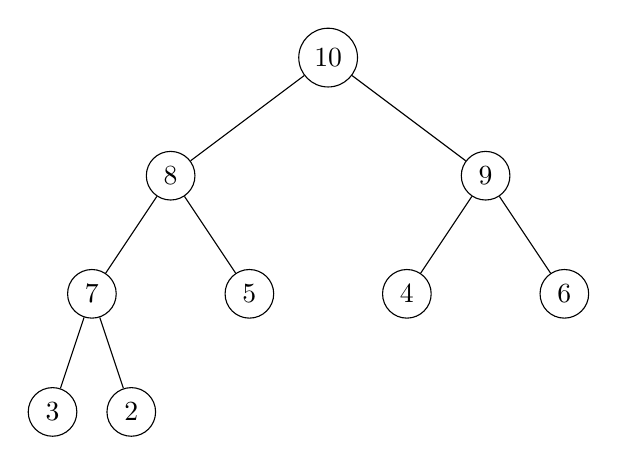
\begin{tikzpicture}[
			level distance=1.5cm,
			level 1/.style={sibling distance=4cm},
			level 2/.style={sibling distance=2cm},
			level 3/.style={sibling distance=1cm}
		]
		\node[circle,draw] {10}
		child {
				node[circle,draw] {8}
				child {
						node[circle,draw] {7}
						child {node[circle,draw] {3}}
						child {node[circle,draw] {2}}
					}
				child {node[circle,draw] {5}}
			}
		child {
				node[circle,draw] {9}
				child {node[circle,draw] {4}}
				child {node[circle,draw] {6}}
			};
	\end{tikzpicture}
\end{figure}

移除堆顶元素(与最后元素交换):

\begin{figure}[H]
	\centering
	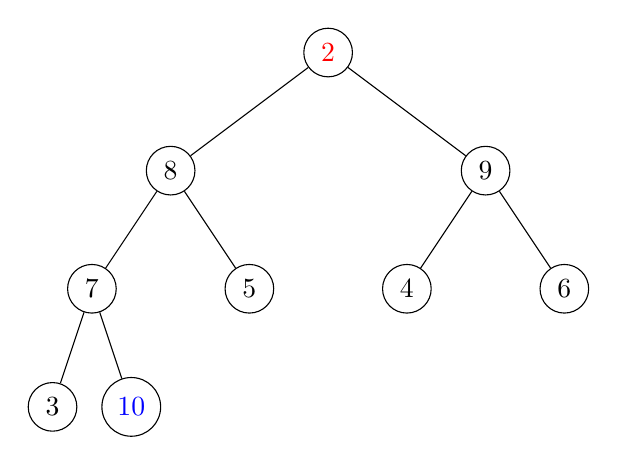
\begin{tikzpicture}[
			level distance=1.5cm,
			level 1/.style={sibling distance=4cm},
			level 2/.style={sibling distance=2cm},
			level 3/.style={sibling distance=1cm}
		]
		\node[circle,draw] {\textcolor{red}{2}}
		child {
				node[circle,draw] {8}
				child {
						node[circle,draw] {7}
						child {node[circle,draw] {3}}
						child {node[circle,draw] {\textcolor{blue}{10}}}
					}
				child {node[circle,draw] {5}}
			}
		child {
				node[circle,draw] {9}
				child {node[circle,draw] {4}}
				child {node[circle,draw] {6}}
			};
	\end{tikzpicture}
\end{figure}

将新的堆顶元素进行下沉,重新调整为大顶堆:

\begin{figure}[H]
	\centering
	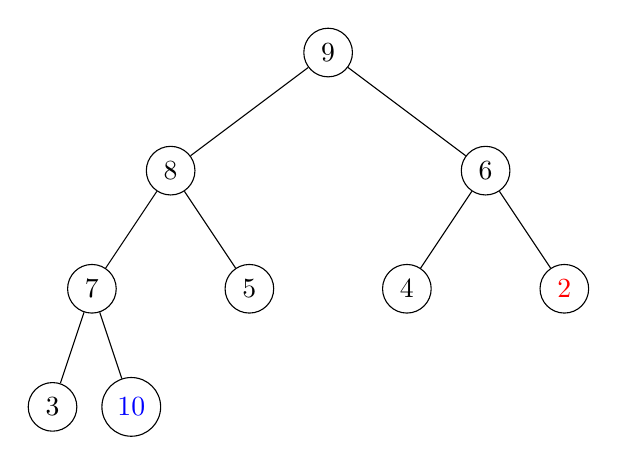
\begin{tikzpicture}[
			level distance=1.5cm,
			level 1/.style={sibling distance=4cm},
			level 2/.style={sibling distance=2cm},
			level 3/.style={sibling distance=1cm}
		]
		\node[circle,draw] {9}
		child {
				node[circle,draw] {8}
				child {
						node[circle,draw] {7}
						child {node[circle,draw] {3}}
						child {node[circle,draw] {\textcolor{blue}{10}}}
					}
				child {node[circle,draw] {5}}
			}
		child {
				node[circle,draw] {6}
				child {node[circle,draw] {4}}
				child {node[circle,draw] {\textcolor{red}{2}}}
			};
	\end{tikzpicture}
\end{figure}

只要反复删除堆顶,反复调节二叉堆,所得到的的集合就成为了一个有序集合。

\begin{figure}[H]
	\centering
	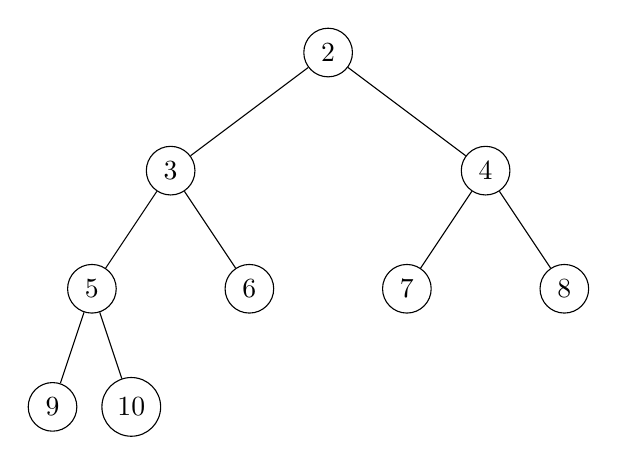
\begin{tikzpicture}[
			level distance=1.5cm,
			level 1/.style={sibling distance=4cm},
			level 2/.style={sibling distance=2cm},
			level 3/.style={sibling distance=1cm}
		]
		\node[circle,draw] {2}
		child {
				node[circle,draw] {3}
				child {
						node[circle,draw] {5}
						child {node[circle,draw] {9}}
						child {node[circle,draw] {10}}
					}
				child {node[circle,draw] {6}}
			}
		child {
				node[circle,draw] {4}
				child {node[circle,draw] {7}}
				child {node[circle,draw] {8}}
			};
	\end{tikzpicture}
\end{figure}

\vspace{0.5cm}

\mybox{堆排序}

\begin{lstlisting}[language=Java]
public static void downAdjust(int[] arr, int parentIndex, int len) {
    // 保存父结点的值,用于最后的赋值
    int temp = arr[parentIndex];
    int childIndex = 2 * parentIndex + 1;

    while(childIndex < len) {
        // 如果有右孩子,且右孩子大于左孩子的值,则定位到右孩子
        if(childIndex + 1 < len 
            && arr[childIndex + 1] > arr[childIndex]) {
            childIndex++;
        }
        // 如果父结点小于任何一个孩子的值,直接跳出
        if(temp >= arr[childIndex]) {
            break;
        }
        // 无需真正交换,单向赋值即可
        arr[parentIndex] = arr[childIndex];
        parentIndex = childIndex;
        childIndex = 2 * childIndex + 1;
    }
    arr[parentIndex] = temp;
}

public static void heapSort(int[] arr) {
    // 把无序数组构建成二叉堆
    for(int i = (arr.length-2) / 2; i >= 0; i--) {
        downAdjust(arr, i, arr.length);
    }

    // 循环删除堆顶元素,移到数组尾部,调节堆产生新的堆顶
    for(int i = arr.length - 1; i > 0; i--) {
        // 最后一个元素和第一个元素交换
        int temp = arr[i];
        arr[i] = arr[0];
        arr[0] = temp;
        // 下沉调整最大堆
        downAdjust(arr, 0, i);
    }
}
\end{lstlisting}

堆排序的空间复杂度为$ O(1) $,因为算法并没有开辟额外的集合空间。\\

至于空间复杂度,假设二叉堆总共有n个元素,那么下沉调整的最坏时间复杂度就等同于二叉堆的高度$ O(logn) $。\\

堆排序的算法步骤分为两部分:

\begin{enumerate}
	\item 把无序数组构建成二叉堆:进行$ n / 2 $次循环,每次循环进行一次下沉调节,因为此步骤的计算规模为$ n/2 * logn $,时间复杂度为$ O(nlogn) $。

	\item 循环删除堆顶元素,移到数组尾部,调节堆产生新堆顶:进行n - 1次循环,每次循环进行一次下沉调节,因此次步骤的计算规模为$ (n-1) * logn $,时间复杂度为$ O(nlogn) $。
\end{enumerate}

综合堆排序的两个步骤,整体时间复杂度为$ O(nlogn) $。

\newpage